\documentclass[9pt,twocolumn,twoside]{../../styles/osajnl}
\usepackage{fancyvrb}
\journal{i524} 

\title{A Report on Apache Apex}

\author[1]{Srikanth Ramanam}


\affil[1]{School of Informatics and Computing, Bloomington, IN 47408, U.S.A.}


\affil[*]{Corresponding authors: srikrama@iu.edu}

\dates{ \today}

\ociscodes{Stream, Processing, YARN, Apache, Apex, Malhar, I524}



% replace this with your url in github/gitlab
\doi{\url{https://github.com/cloudmesh/sp17-i524/raw/master/paper2/S17-IR-2028/report.pdf}}

\begin{abstract}
Apache Apex is a Hadoop YARN native big data processing platform with both stream and batch processing capabilities. This paper explores the architecture, functioning and competition of Apache Apex.
\newline
\end{abstract}

\setboolean{displaycopyright}{true}

\begin{document}

\maketitle

\section{Introduction}
 Apex is an enterprise-grade stream and batch processing platform for the  Apache Hadoop ecosystem \cite{www-asfblog}. It was initially developed by DataTorrent as the core engine for RTS,a data processing and analytics platform. Apex was submitted to Apache incubator in 2015 \cite{www-datatorrentapex}. Later several enterprises like CapitalOne, DirecTV, General Electric, Apple and Silver Spring Networks joined its open source community. Apache Apex was first released in 2016. 

Apache Apex is built over YARN and is compatible with existing Hadoop platforms, allowing users to leverage their previous Hadoop investments and applications \cite{www-apacheapexblog}. According to Apache Apex website \cite{www-apacheapexsite}, " it processes big data in-motion in a way that is highly scalable, highly performant, fault tolerant, stateful, secure, distributed, and easily operable".
Apex automatically handles operational aspects like state management, fault tolerance, scalabilty etc \cite{www-apacheapexdoc}. It also provides a simple API that supports Java, facilitating easy development and widespread adoption \cite{www-apacheapexdoc}. It also has a REST API facilitating compatibility with popular web technologies. Apache Apex also has a metrics API that allows users to monitor various aspects of operators in real time.







\section{Components}
Apache Apex has two main components. They are Apex Core and Apex Malhar \cite{www-apacheapexwiki}.
\subsection{Apex Core}
Apex Core is the framework for building distributed stream processing and analytics applications on Hadoop. It also enables building of unified batch and stream processing applications.
\subsection{Apex Malhar}
Malhar provides a library of operators that perform widely used functionality. These reusable blocks reduce the amount of coding required to build applications and enable users to speed up application development. Operators offered by are mainly of two types
\subsubsection{Input/Output Operators}
Input/Output operators: These operators offer connectivity with a variety of existing data sources.
\subsubsection{Compute Operators}
Compute Operators: These operators offer functionality of Machine Learning, Stats and Math, Pattern Marching, Query and Scripting, Stream manipulators, Parsers and UI \& Charting.
\begin{figure}[ht!]
\centering
\fbox{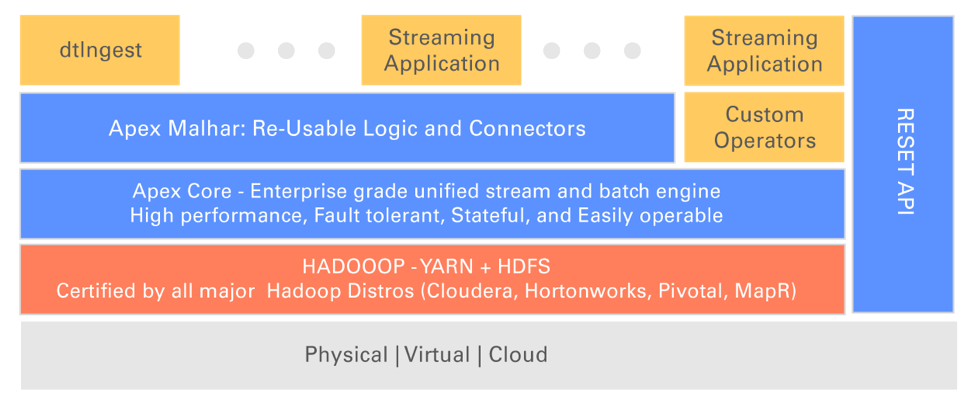
\includegraphics[width=\linewidth]{images/apache-apex-easily-reused.png}}
\caption{Apache Apex Components \cite{www-apacheapexblog}}
\label{fig:Apache Apex Components}
\end{figure}




\section{Architecture}

Operators are the basic blocks of Apex applications. A streaming application is built using in-built or custom operators are connected to form a DAG (Directed Acyclic Graph) using streams. 
\begin{figure}[ht!]
\centering
\fbox{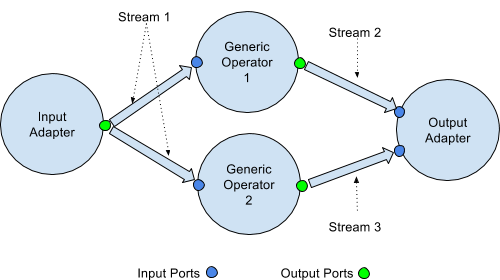
\includegraphics[width=\linewidth]{images/DAG.png}}
\caption{Apex Application DAG \cite{www-apacheapexappdevdoc}}
\label{fig:Apex Application DAG}
\end{figure}



\section{Application Development}
Apex applications can be written in Java using any IDE supporting Java like Eclipse.
Other prerequisites include Apache Maven 3.0., Apache Apex, Apache Malhar \cite{www-apacheapexappdevdoc}.

\subsection{Operators}
Operators are independent units of logical operations that either contribute to a part of or a whole business use case. An operator has an input port to receive data tuples and an output port to send data tuples to another operator  or external system \cite{www-apacheapexoperatordoc}.
\subsubsection{Types of Operators \cite{www-apacheapexoperatordoc}}
\begin{itemize}
  \item Input Adapter:  An operator at the beginning of the DAG to receive data from an external system.
  \item  Generic Operator: Accepts tuples from previous operator in DAG and does some processing task and outputs the processed data to another operator.
  \item An operator at the end of a DAG and outputs the data tuples to an external system. 
  
\end{itemize}

\subsubsection{Operator API \cite{www-apacheapexoperatordoc}}
\begin{itemize}
  \item setup() initializes the operator.
  \item process()  performs the core processing operations on data tuples and gets triggered when tuples are received.
  \item beginWindow()  and endWindow() are used for pre and post processing steps.
  \item teardown() shuts down the operator and releases the resources held by the operator.
\end{itemize}
\subsection{Directed Acyclic Graph}
A Directed Acyclic Graph(DAG), is constructed to accomplish a business task using several operators connected through streams \cite{www-apacheapexappdevdoc}. A stream is a sequence of data tuples.
To construct a DAG, operators are added using dag.addOperator(args) while streams are added using dag.addStream(args). Other configurations related to YARN can also be added to DAG \cite{www-apacheapexinslideshare}.

\subsection{Package}
Apex applications are assembled and shared using Apache Apex Packages, which are zip files with all necessary files to launch those applications.
Apache Apex Packages are created using Maven.                 
First a Maven project is created with path to the application code. 
Then a mvn package command creates an application package in the target package.
Zip structure of a mvn package consists of app with jar files of the DAG code, lib with jar files of dependencies, conf with preset configurations, META-INF consisting of meta information in files and resources for other files \cite{www-apacheapexpackagedoc}.
\begin{figure}[ht!]
\centering
\fbox{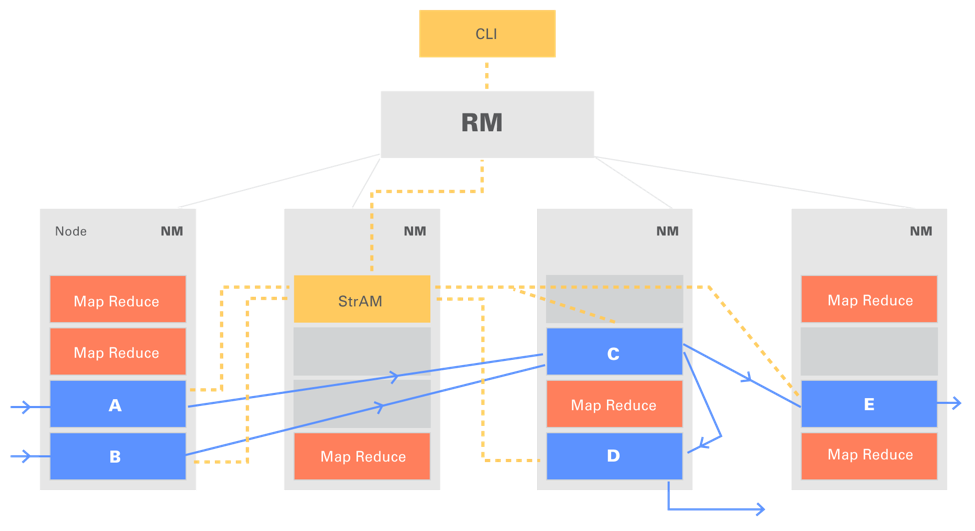
\includegraphics[width=\linewidth]{images/apex-application-in-hadoop-cluster.png}}
\caption{Apache Apex Application Example \cite{www-apacheapexblog}}
\label{fig:Apache Apex Application Example}
\end{figure}


\section{Functioning}
Apache Apex applications are built as DAGs consisting of operators and streams. These applications  are packaged, shared and deployed over Hadoop clusters.

\subsection{Fault tolerance and Recovery}
The states of operators and application master are checkpointed regularly to a persistent store like HDFS \cite{www-apacheapexintroslideshare}.
Failed operators are automatically detected through continuous monitoring \cite{www-apacheapexintroslideshare}.
When a failure occurs, the checkpointed states of operators are used to revive the application \cite{www-apacheapexintroslideshare}.
Data can be made to replay from the checkpointed state of the operator after recovery preventing data loss \cite{www-apacheapexintroslideshare}.

\subsection{Compatibility}
Apache Apex is also compatible with several popular data file systems, message systems and database systems through connectors provided by Malhar. 
They are shown in the below figure.
\begin{figure}[ht!]
\centering
\fbox{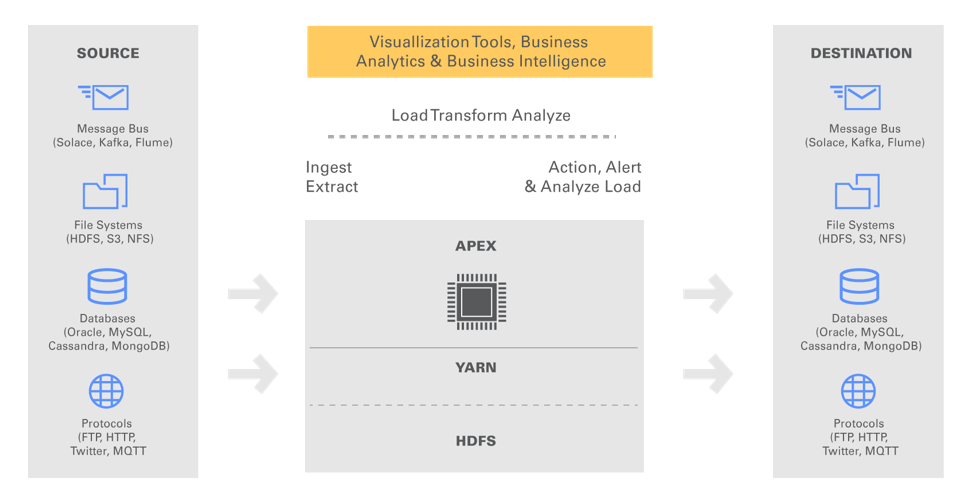
\includegraphics[width=\linewidth]{images/apache-apex-ease-of-integration.png}}
\caption{Apache Apex Interoperability\cite{www-apacheapexblog}}
\label{fig:Apache Apex Interoperability}
\end{figure}




\section{User Interface}
A command line interface called Apex CLI is available for Apache Apex \cite{www-apacheapexclidoc}.
It can be launched with command  apex. help command is available for all commands to obtain information and syntax.


Apache Apex's REST, Java API's can be integrated with commonly used existing web technologies to create web interfaces for visual analytics. Data Torrent also offers RTS platform, built on Apex, which provides visualization with several real-time dashboards that help monitor streaming applications \cite{www-apacheapexintroslideshare}.

\section{License and Pricing}
Apache Apex is a free and open source software. It is licensed under Apache License 2.0 \cite{www-apacheapexsite}.  


\section{Competition}
Some of the competitors of Apache Apex for stream processing and analytics are \cite{www-apacheapexcompetition}:
\subsection{Apache Spark}
 This is a large-scale data processing engine that also offers stream processing \cite{www-apachesparksite}. But this is not a pure streaming engine as it accomplishes the same through micro-batching, fast execution of batches on small sets of data. 
\subsection{Apache Flink}
Apache Flink is an open-source stream processing framework that processes streams in real-time \cite{www-apacheapexflink}. This is almost similar to Apex but not as widely used.
\subsection{Apache Storm}
This is a free and open source distributed real-time computation system \cite{www-apachestormsite}. This is fast but not stateful like Apache Apex.
\subsection{Apache Samza}
Apache Samza is a distributed stream processing framework \cite{www-apachesamzasite}.It was first developed by LinkedIn and later opensourced \cite{www-newsstacksamza}. It is built on top of Apache Kafka \cite{www-apachekafkasite}, a distributed streaming platform. It provides stateful streaming capabilities \cite{www-newsstacksamza}. It has great compatibility with Kafka \cite{www-newsstacksamza}. Streaming applications can be built in such that Kafka consumes the data processed by Samza \cite{www-newsstacksamza}.
\section{Users}
With its stream processing capabilities, Apache Apex facilitates building large scale real-time analytics applications. Enterprises like GE, PubMatic, SilverSpring Networks are using Apex based streaming solutions \cite{www-apacheapexinslideshare}. 
\section{Conclusion}
Apache Apex is an open source YARN(Hadoop 2.0)-native platform \cite{www-apacheapexwiki}. It unifies stream and batch processing. It can be used for processing both streams of data and static files making it more relevant in the context of present day internet and social media. It is aimed at leveraging the present Hadoop platform and reducing the learning curve for development of applications over it. It is aimed at It can used through a simple API. It enables reuse of code by not having to make drastic changes to the applications by providing interoperability with existing technology stack. It leverages the existing Hadoop platform investments.



\section*{Acknowledgements}

This paper has been written as part of a class assignment for the course: 
I524: Big Data Software and projects, Spring 2017, School of Informatics and computing, Indiana University, Bloomington.
Special thanks to Professor Gregor von Laszewski, Dimitar Nikolov and all associate instructors for guiding through the process of writing this paper.


% Bibliography

\bibliography{references}
 
\end{document}









